\documentclass[a4paper,12pt]{report}

\usepackage{alltt, fancyvrb, url}
\usepackage{graphicx}
\usepackage[utf8]{inputenc}
\usepackage{float}
\usepackage{hyperref}

% Questo commentalo se vuoi scrivere in inglese.
\usepackage[italian]{babel}

\usepackage[italian]{cleveref}

\title{Meta-relazione per\\``esame''}

\author{Giosuè Giocondo Mainardi}
\date{\today}


\begin{document}

\maketitle

\begin{abstract}
Questo è l'abstract, la struttura della relazione è \textit{indicativa}.

L'uso di \LaTeX{} è vantaggioso per chi ama l'approccio ``what you mean is what you get'', ossia voglia disaccoppiare il contenuto dall'effettivo rendering del documento, accollando al motore \LaTeX{} l'onere di produrre un documento gradevole con la struttura ed il contenuto forniti.
%
Chi non volesse installare l'ambiente di compilazione in locale può valutare l'utilizzo dell'applicazione web \href{https://www.overleaf.com/}{Overleaf}.
%

Esempio di footnote con MermaidJS\footnote{\url{https://mermaid.live/}} o PlantUML \footnote{\url{https://plantuml.com/}}.
\end{abstract}

\tableofcontents

\chapter{Analisi}

\textit{Esempio in corsivo.}
\section{Requisiti}

Per enfatizzare \emph{requisiti}.

\subsection*{Sottosezione con elenco}
\begin{itemize}
	\item primo punto
	\item secondo punto
	\item terzo punto
\end{itemize}

\subsection*{Sottosezione importante: Esempio}

\section{Sezione esempio}

Anche una parte in \textbf{grassetto.}

\subsection*{Esempio}
Esempio immagine \Cref{img:example}.

\begin{figure}[H]
\centering{}
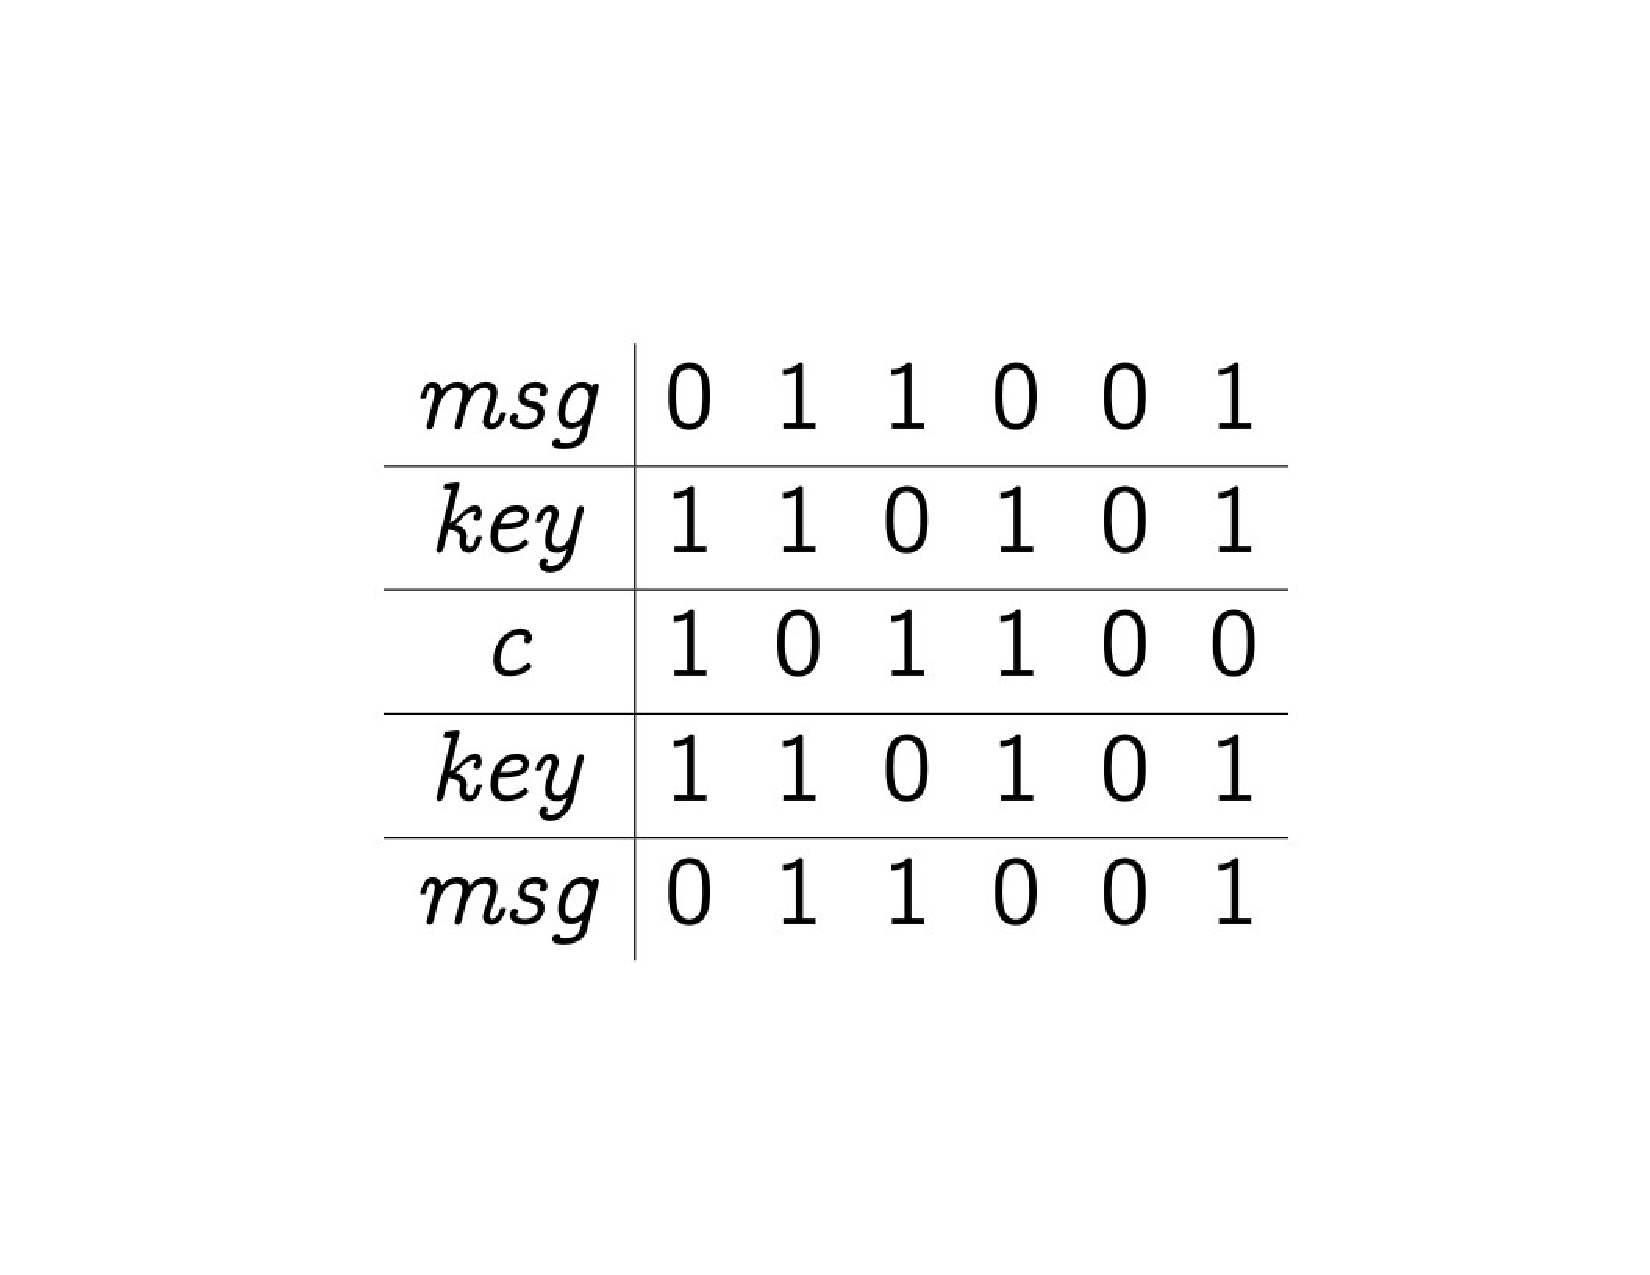
\includegraphics{img/example_img.pdf}
\caption{descrizione immagine.}
\label{img:example}
\end{figure}

\chapter{Capitolo 2}

\section{Sezione 1 Capitolo 2}

Contenuto.

\subsection*{Esempio}
Conseguentemente, GLaDOS è un ``observable'' per Output.

Qua esempio di immagine inserita sul posto.

\begin{figure}[h]
\centering{}
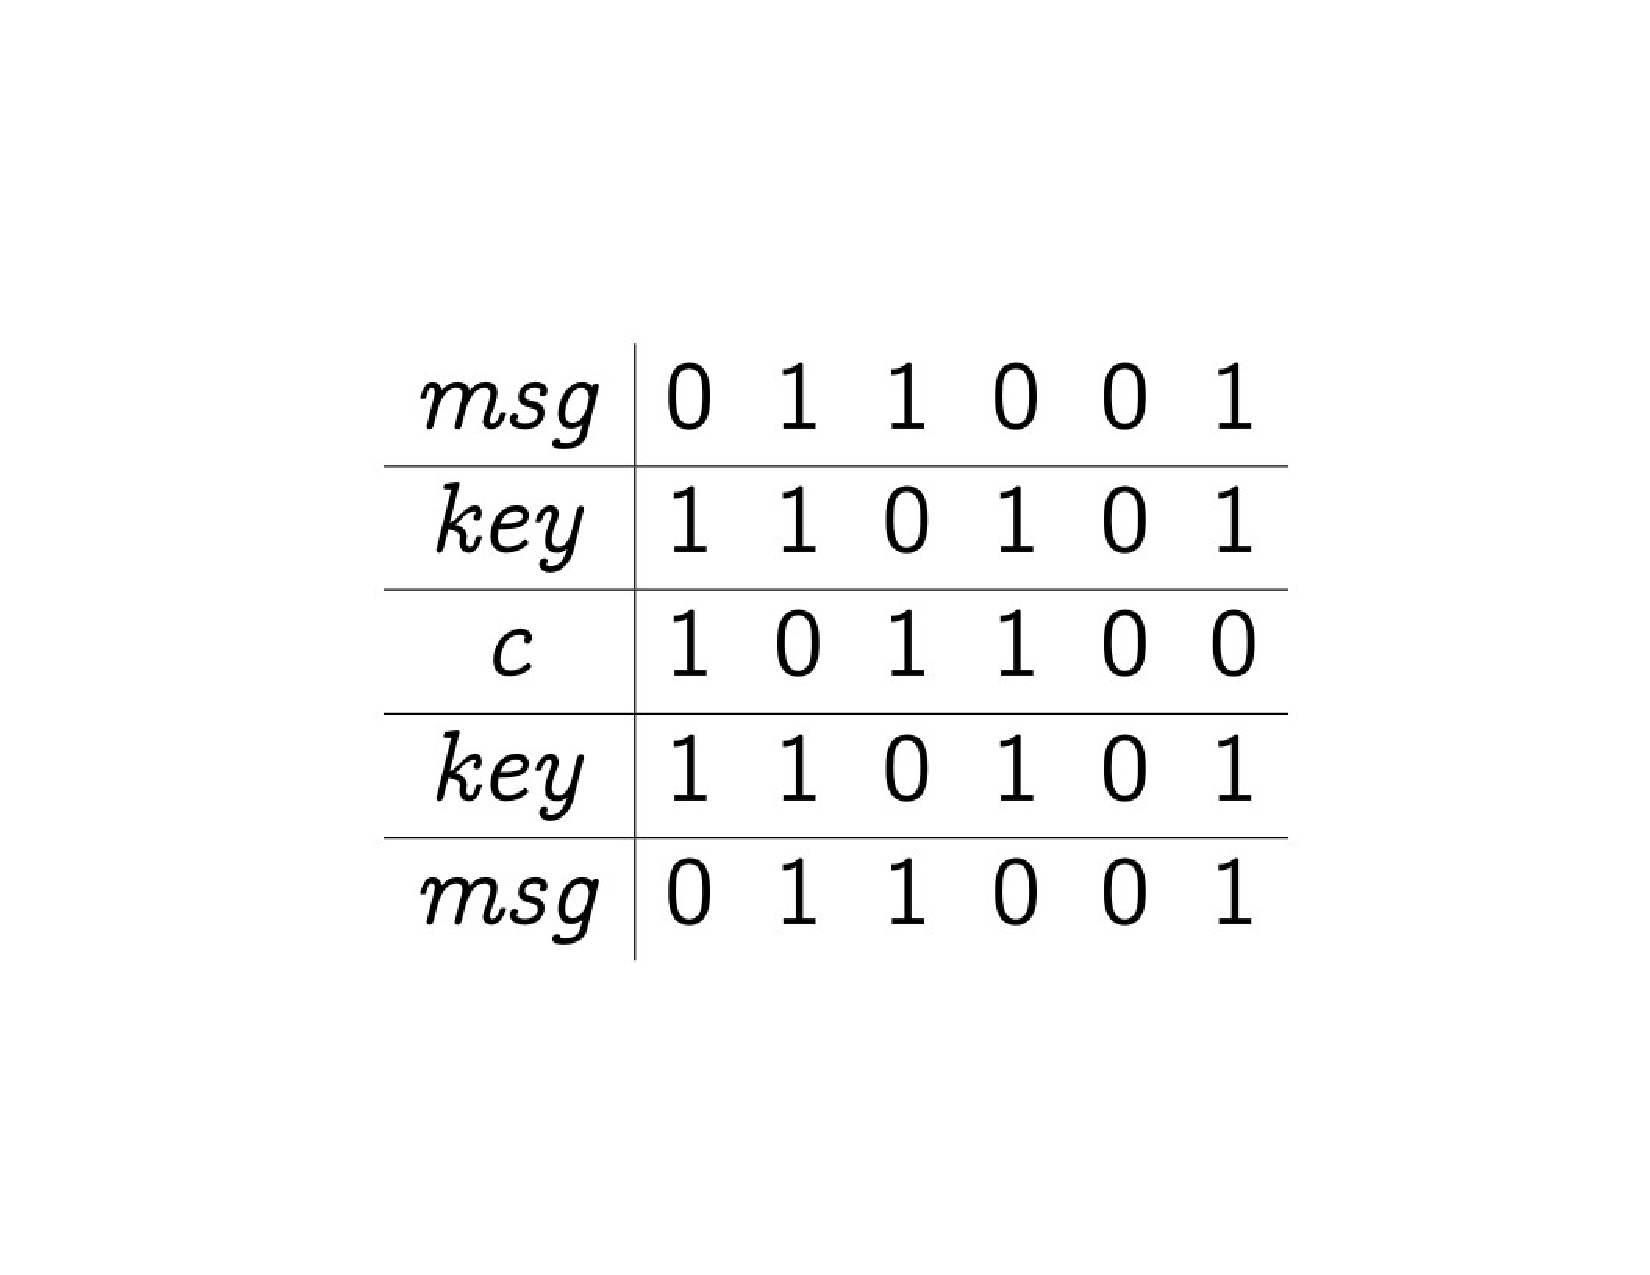
\includegraphics[width=\textwidth]{img/example_img.pdf}
\caption{L'interfaccia \texttt{GLaDOS}.}
\label{img:example2}
\end{figure}

\section{Altra sezione}

\textbf{Sottotesto in grassetto}.

\subsection*{Esempio minimale}

\subsubsection{Sotto sotto sezione con paragrafi}

\paragraph{Paragrafo1} Contenuto.

\paragraph{Paragrafo Risposta 1} Contenuto \textit{paragrafo}, con riferimento immagine
\Cref{img:example}: e anche \texttt{Scrittura unicode}.

\chapter{Capitolo 3}
\section{Sezione}

Contenuto

\subsection{Esempio con sottosezioni e permalink}

\subsubsection{Utilizzo di \texttt{LoadingCache} dalla libreria Google Guava}

Permalink: \url{https://github.com/AlchemistSimulator/Alchemist/blob/d8a1799027d7d685569e15316a32e6394632ce71/alchemist-incarnation-protelis/src/main/java/it/unibo/alchemist/protelis/AlchemistExecutionContext.java#L141-L143}

\subsubsection{Utilizzo di \texttt{Stream} e lambda expressions}

Usate pervasivamente. Il seguente è un singolo esempio.
Permalink: \url{https://github.com/AlchemistSimulator/Alchemist/blob/d8a1799027d7d685569e15316a32e6394632ce71/alchemist-incarnation-protelis/src/main/java/it/unibo/alchemist/model/ProtelisIncarnation.java#L98-L120}

\subsubsection{Scrittura di metodo generico con parametri contravarianti}

Permalink: \url{https://github.com/AlchemistSimulator/Alchemist/blob/d8a1799027d7d685569e15316a32e6394632ce71/alchemist-incarnation-protelis/src/main/java/it/unibo/alchemist/protelis/AlchemistExecutionContext.java#L141-L143}

\chapter{Capitolo finale}

In quest'ultimo capitolo si tirano le somme del lavoro svolto e si delineano eventuali sviluppi
futuri.

\section{Sezione di commenti finali}

\textbf{È richiesta una sezione per ciascun membro del gruppo, obbligatoriamente}.

\appendix
\chapter{Capitolo appendice 1}

Contenuto.

\chapter{Capitolo appendice 2}

Contenuto.

\bibliographystyle{alpha}
\bibliography{report-template}

\end{document}
